\documentclass{article}
\usepackage{amsfonts}          % Para las negrita de pizarra
\usepackage{indentfirst}       % Para que quede mas lindo el formateo
\usepackage{graphicx}          % Para graficos
\usepackage{minted}            % Para poner codigo y que quede con sintaxis fachera
\usepackage{hyperref}          % Para meter hipervinculos
\usepackage[dvipsnames]{xcolor}% Para usar colores
\usepackage{hhline}            % Mas configuracion para las líneas en tablas
\usepackage{amsmath}           % Agregado para tags de ecuaciones
\usepackage{xcolor}            % Coloreado de ecuaciones
\usepackage{quoting, xparse}   % Usado para citar
% \usepackage{svg}               % Para usar imagenes svg que se ven lindas independientemente del zoom. WARNING REQUIERE DE INKSCAPE. Tal vez no vale la pena
\usepackage{amsmath}

\graphicspath{ {./images/} }

\newcommand{\docuPy}{%
  {\href{https://wiki.python.org/moin/TimeComplexity}{documentación oficial}}
  }%

  % Comandos para facilitar el citado
  % Fuente: https://tex.stackexchange.com/a/391739/273865
\NewDocumentCommand{\bywhom}{m}{% the Bourbaki trick
  {\nobreak\hfill\penalty50\hskip1em\null\nobreak
   \hfill\mbox{\normalfont(#1)}%
   \parfillskip=0pt \finalhyphendemerits=0 \par}%
}

\begin{document}

\begin{titlepage}
  \vspace*{1cm}

  \begin{center}
    {\Huge{Trabajo Práctico 3: Problemas NP-Completos para la defensa de la Tribu del Agua}}
  \end{center}

  \vspace{0.4cm}

  \begin{center}
    {\LARGE{Facultad de Ingeniería de la Universidad de Buenos Aires}}\\
    \vspace{0.3cm}
    {\Large{Teoría de Algoritmos}}\\
    \vspace{0.3cm}
    {\large{Cátedra Buchwald-Genender}}\\
  \end{center}

  \vspace{0.8cm}
  \begin{center}
    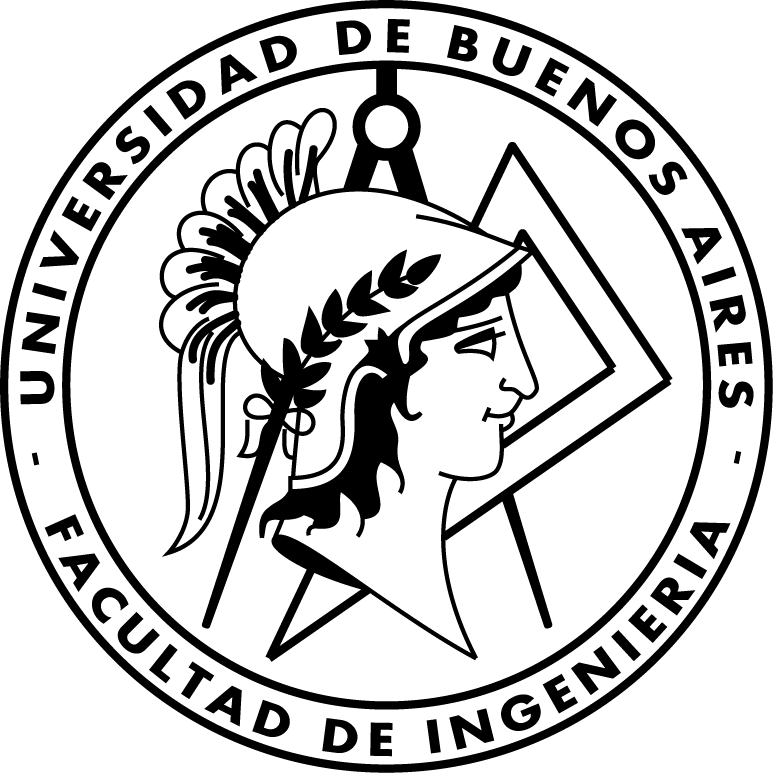
\includegraphics[scale=0.8]{Logo-fiuba}
  \end{center}

  \vspace{1.4cm}
  \begin{center}

    {\begin{minipage}[t]{.32\textwidth}
        \begin{center}
          Gómez Belis, Sofía\\
          {\small{Padrón: 109358}}\\
          {\small{email: sgomezb@fi.uba.ar}}
        \end{center}
          \end{minipage}
          \begin{minipage}[t]{.32\textwidth}
        \begin{center}
          Llanos Pontaut, Valentina\\
          {\small{Padrón: 104413}}\\
          {\small{email: vllanos@fi.uba.ar}}\\
        \end{center}
      \end{minipage}
      \begin{minipage}[t]{.32\textwidth}
        \begin{center}
          Orsi, Tomas Fabrizio\\
          {\small{Padrón: 109735}}\\
          {\small{email: torsi@fi.uba.ar}}
        \end{center}
      \end{minipage}}

  \end{center}
\end{titlepage}

\renewcommand*\contentsname{Indice}
\tableofcontents
\pagebreak

\section{Introducción}
\subsection{Descripción y objetivo}

Continuando con el ataque de la Nación del Fuego sobre el resto de las naciones, esta vez es la Tribu del Agua la que requiere de nuestra ayuda para defenderse. 

Cada maestro agua tiene una fuerza o habilidad positiva $x_i$, y contamos con el conjunto de todos los valores $(x_i, x_2, \dots, x_n)$. Basándonos en estos, el maestro Pakku desea separar los maestros en \texttt{k} grupos $(S_1, S_2, \dots, S_k)$ parejos tal que cuando un grupo se canse, entrará el siguiente en el combate, obteniendo un ataque constante que les permita salir victoriosos, aprovechando también la ventaja del agua por sobre el fuego.

Para que los grupos estén lo más parejos posibles, nos han encomendado minimizar la adición de los cuadrados de las sumas de las fuerzas de los grupos:

$$
\min \sum_{i=1}^{k} \left( \sum_{x_j \in S_i} x_j \right)^2
$$

En este trabajo desarrollaremos algoritmos de backtracking, programación lineal y posibles aproximaciones buscando resolver el problema planteado con el objetivo de ayudar a los maestros de la Tribu del Agua a derrotar a la Nación del Fuego.

\section{Demostración de problema NP-Completo}

Los problemas NP-Completos son los problemas más difíciles de NP. Cualquier problema en NP puede ser reducido a uno NP-Completo.

Para demostrar que el problema de la Tribu del Agua es NP-Completo, primero debemos demostrar que se encuentra en NP. Posteriormente, si logramos hacer una reducción polinomial de un problema NP-Completo a éste, entonces esto implica que también se trata de un problema NP-Completo. Ésto se debe a que la reducción $Y \leq_p X$ implica que la dificultad de resolver \texttt{Y} se reduce polinomialmente a la dificultad de resolver \texttt{X}, o que \texttt{X} es al menos tan difícil de resolver como \texttt{Y}. Si \texttt{Y} es un problema NP-Completo, entonces \texttt{X} es al menos tan difícul de resolver como un problema NP-Completo.

Para realizar la demostración y la reducción, necesitamos basarnos en el problema de decisión:

Dados una secuencia de \texttt{n} fuerzas de maestros agua $(x_i, x_2, \dots, x_n)$, y dos números \texttt{k} y \texttt{B}, ¿existe una partición en \texttt{k} subgrupos $(S_1, S_2, \dots, S_k)$ tal que:

$$
\sum_{i=1}^{k} \left( \sum_{x_j \in S_i} x_j \right)^2 \leq B
$$

y cada elemento $x_i$ esté asignado a solamente un grupo?
\subsection{Problema NP}

Un problema se encuentra en NP si existe un certificador eficiente para el mismo. Es decir, si puede ser verificado o validado en tiempo polinomial. 

Tenemos los siguientes datos:
\begin{itemize}
    \item Habilidades de los maestros $\rightarrow$ se presentan en forma de tupla (nombre maestro, fuerza)
    \item Cantidad de subconjuntos $\rightarrow$ \texttt{k}
    \item Cota del coeficiente $\rightarrow$ \texttt{B}
    \item Resultado a validar $\rightarrow$ subconjuntos $S_i$ que contienen los nombres de los maestros del grupo correspondiente
\end{itemize}

También tenemos las siguientes restricciones:
\begin{itemize}
    \item Cada maestro debe estar asignado a un solo grupo
    \item El resultado debe contener \texttt{k} grupos
    \item La sumatoria resultante debe ser a lo sumo \texttt{B} 
\end{itemize}

Dados estos datos y restricciones, proponemos el siguiente certificador.
\inputminted[linenos, firstline=1, lastline=31]{python}{codigo/certificador_eficiente.py}

Para que el verificador presentado pueda ser considerado un certificador eficiente, debe ejecutarse en tiempo polinomial. Por lo tanto, procedemos a explicar y justificar la complejidad del código.

Realizamos operaciones aritméticas, asignaciones y verificaciones. Todas estas son operaciones $O(1)$ puesto que consumen tiempo constante según la \docuPy. Recorremos dos veces la lista de maestros y habilidades con diferentes propósitos. Como contiene \texttt{n} tuplas, cada ciclo \texttt{for} tiene un costo $O(n)$. Con el objetivo de obtener la adición de los cuadrados de las sumas de las fuerzas de los grupos y compararla con \texttt{B}, tenemos dos ciclos anidados. El segundo recorre los maestros de un grupo que, en el peor caso, son \texttt{n}. Esto se realiza \texttt{k} veces, por lo que en total es $O(k \times n)$.

Entonces,

$$
T(n) = O(1) + 2 \cdot O(n) + O(k \times n) = O(k \times n)  
$$

En el peor caso, $k = n$ y

$$
T(n) = O(n \times n) = O(n^2)
$$

Ambas cotas, $O(k \times n)$ y $O(n^2)$ conllevan tiempo polinomial. Por lo tanto, podemos afirmar que existe un certificador eficiente para el problema de la Tribu del Agua y entonces este problema está en NP.

\subsection{Reducción}

\section{Complejidad algorítmica}
\subsection{Complejidad lectura de archivos}
\subsection{Complejidad algoritmo de Backtracking}
\subsection{Complejidad algoritmo de programación lineal}
\subsection{Complejidad algoritmo de aproximación}

\subsection{Efecto de las variables sobre el algoritmo}

\section{Ejemplos de ejecución}
\label{sec:ejemplos}
\section{Mediciones de tiempo}
\label{sec:medTiempo}
\subsection{Algoritmo de backtracking}
\subsection{Algoritmo de programación lineal}
\subsection{Algoritmo de aproximación}


\section{Conclusión}


\end{document}
